%%%%%%%%%%%%%%%%%%%%%%%%%%%%%%%%%%%%%%%%%%%%%%%%%%%%%%%%%%%%%%%%%%%
%    INSTITUTE OF PHYSICS PUBLISHING                              %
%%%%%%%%%%%%%%%%%%%%%%%%%%%%%%%%%%%%%%%%%%%%%%%%%%%%%%%%%%%%%%%%%%%
\documentclass[10pt]{iopart}
\usepackage[sort, compress]{cite}   
\usepackage{bm}
\usepackage{siunitx}
\usepackage{units}
\usepackage{graphicx}   % Graphikpaket (fuer PNG,GIF,JPG)
\usepackage[pdfstartview=FitH,                     % Oeffnen mit fit width
                   breaklinks=true,                         % Umbrueche in Links, nur bei pdflatex default
                   bookmarksopen=true,                % aufgeklappte Bookmarks
                   bookmarksnumbered=true,        % Kapitelnummerierung in bookmarks
                   pdfprintscaling=None,                % Default-Einstellung zum Drucken: nicht skaliert
                   pdfduplex=DuplexFlipLongEdge, % Default-Druck-Einstellung: Duplex
					hidelinks,                   
                   ]{hyperref}

\newcommand{\gguide}{{\it Preparing graphics for IOP Publishing journals}}
%Uncomment next line if AMS fonts required
%\usepackage{iopams}  
\begin{document}

\title[Miniaturized fourier-plane fiber-scanner for OCT endoscopy]{Miniaturized fourier-plane fiber-scanner for OCT endoscopy}

\author{Authors}

\address{Address}
\ead{email}
\vspace{10pt}
\begin{indented}
\item[]February 2014
\end{indented}

\begin{abstract}


\end{abstract}
% Uncomment for PACS numbers
%\pacs{00.00, 20.00, 42.10}
%
% Uncomment for keywords
%\vspace{2pc}
%\noindent{\it Keywords}: XXXXXX, YYYYYYYY, ZZZZZZZZZ
%
% Uncomment for Submitted to journal title message
%\submitto{\JPA}
%
% Uncomment if a separate title page is required
%\maketitle
% 
% For two-column output uncomment the next line and choose [10pt] rather than [12pt] in the \documentclass declaration
\ioptwocol
%

%%%%%%%%%%%%%%%%%%%%%%%%%%%%%%%%%%%%%%%%%%%%%%%%%%%%%%%%%%%%%%%%%%%%%%%%
\section{Introduction}
%%%%%%%%%%%%%%%%%%%%%%%%%%%%%%%%%%%%%%%%%%%%%%%%%%%%%%%%%%%%%%%%%%%%%%%%
The aging of our society is encouraging an institutional effort towards the early detection of diseases \cite{Fendrich2007}. As checkups and screenings become more common, there is a need for better, less invasive diagnostic methods that reduce the risks and discomfort of the patient. 

This is the goal of optical biopsy: a collective name for advanced endomicroscopy methods allowing real-time, \textit{in-situ} diagnosis of tissue malignancies without the need of excision and histopathological analysis. One of the enabling technologies for optical biopsy is optical coherence tomography (OCT), an imaging method that allows the retrieval of depth information of a sample from its backscattered light.  Due to its non-invasive nature and long working distance it found its first uses in ophtalmology, but it is currently under research in an expanding variety of endoscopic applications. 

The first endoscopic OCT implementations were restricted to side viewing, single modality OCT catheter-endoscopes that sampled the tissue by translating \cite{Feldchtein1998} or rotating \cite{Tearney1994, Tearney1996} the probe to acquire \textit{in-vivo} 2D cross sections through the lumen. This scanning method, displacing the entire catheter, resulted in poor dimmensional accuracy and speed. This can be solved by performing the scanning within the probe. Earlier works demonstrated this approach using Coherent Fiber Bundles (CFB) to create forward viewing endoscopes, where individual cores in the CFB were scanned sequentially to perform OCT imaging. The advantage of this method is that the scanning mechanism is located outside the body, which allows the endoscope tip to be relatively compact. As a tradeoff, the final image quality acquired with such systems suffer from poor SNR (signal-to-noise ratio) due to the CFB’s multi-mode behavior and distinct inter-core coupling \cite{Xie2005}. Furthermore, these systems are unsuitable for flexible endoscopes due to the rigidity of CFBs.

A new mechanism, the \textit{image plane fiber scanner} \cite{Seibel2001}, allowed forward-viewing video endoscopes with diameters under \SI{1}{\milli\meter} within thin, flexible catheters. 
These devices use the concept of mechanical resonance to amplify the subtle movement of a piezoelectric actuator into a large displacement of the tip of an optical fiber oscillating in its first resonant mode. If the tip of the scanner is placed at the image plane of an optical system, as depicted in figure \ref{fig:fiberScanner}, the lateral displacement of the fiber will image the object plane. 
\begin{figure}[h!]\centering 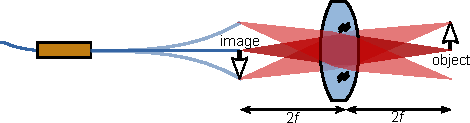
\includegraphics{figures/fiberScanner.pdf}
      \caption{Working principle of an image plane fiber scanner}
      \label{fig:fiberScanner}
\end{figure}

Although this scanning method can be extended to OCT \cite{Lurie2015}, the high resonance frequency of the fiber, typically in the range of several kilohertz, make it difficult to sample the spectral information fast enough. Although it is possible to decrease the resonance frequency by using a longer fiber or a weight on its tip \cite{Moon2010}, this approach significantly increases the length of the device. 

This work demonstrates a novel topology of fiber scanner which is optimized for OCT, namely the fourier plane fiber scanner. This topology enables shorter OCT endoscopes with higher spatial sampling with shorter rigid tip length. Furthermore, it performs telecentric scanning, which reduces vigneting in the outer areas of the image and avoids distortions in the reconstructed 3D images.


%%%%%%%%%%%%%%%%%%%%%%%%%%%%%%%%%%%%%%%%%%%%%%%%%%%%%%%%%%%%%%%%%%%%%%%%
\section{Requirements of OCT scanners}
%%%%%%%%%%%%%%%%%%%%%%%%%%%%%%%%%%%%%%%%%%%%%%%%%%%%%%%%%%%%%%%%%%%%%%%%

The presented probe is optimized for Swept-Source Optical Coherence Tomography (SS-OCT). This type of OCT uses a Michelson interferometer in which the reference arm is fixed while the sample arm illuminates a portion of a sample and collects the backscattered light, as depicted in \autoref{fig:OCT}. This light originates from a narrowband laser with the ability to tune its wavenumber. 


The optical path difference between each layer of the sample and the reference arm in the interferometer induces a change in the intensity detected by the photodiode. The variation of this intensity versus the wavenumber of the laser creates an interferogram, whose Fourier transformation encodes the reflectivity information a transversal column of the sample, named A-scan. This process can be performed in real time to speeds typically around 100 kHz. By scanning the position of the laser beam, it is possible to reconstruct 3D volumes of the sample.

\begin{figure}[h!]\centering 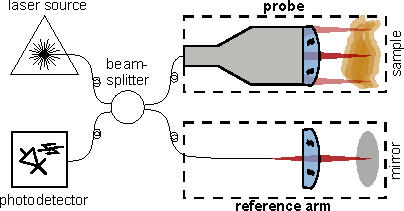
\includegraphics{figures/OCTsetup.pdf}
      \caption{Simplified fiber-based swept-source OCT system. Light originating from a swept-source laser is coupled to an interferometer, where the optical path difference between the sample and the reference arm creates an interferogram measured with a photodetector.}
      \label{fig:OCT}
\end{figure}

The requirements of the optical system and the scanner can be pointed out from the previous description: 

First, in order to obtain volumetric images, a 2D scanner has to be integrated into a compact probe. As the sampling rate of OCT systems is typically constrained, the scanner should displace the focus position slow enough so that the spatial sampling $k_{sampling}$ is at least double than the maximum resolvable spatial frequency of the optical system $k_{opt}$,
\begin{equation}
k_\mathrm{sampling} > 2 \ k_\mathrm{opt}.
\end{equation}
and thus fulfilling the Nyquist criterium.

Second, the depth of field (DoF) of the focused beam should be several millimeters to enable a long penetration depth, usually in the 2-4 mm range. Thus, a low numerical aperture (NA) is preferred, ranging from 0.02 to 0.05.

Further characteristics are also desirable: smaller probe diameters enable their use in new applications, shorter probes enable flexible-tip endoscopes which can orient the field of view, and telecentric imaging ease the quantitative analysis of the acquired data.


%%%%%%%%%%%%%%%%%%%%%%%%%%%%%%%%%%%%%%%%%%%%%%%%%%%%%%%%%%%%%%%%%%%%%%%%
\section{Fourier plane fiber scanners}
%%%%%%%%%%%%%%%%%%%%%%%%%%%%%%%%%%%%%%%%%%%%%%%%%%%%%%%%%%%%%%%%%%%%%%%%


The scanner proposed in this work fulfills the above-mentioned requirements by implementing a Fourier plane fiber scanner (FPFS) topology. 

Compared with the image plane fiber scanner, depicted in \autoref{fig:fiberScanner}, the FPFS has a GRIN lens glued to the tip of the fiber, significantly reducing the resonance frequency of the vibrating cantilever and also collimating the laser beam. The fiber scanner is then positioned such that the lateral and angular movement of the scanner behaves as the beam angles that can be observed in the collimated region of a classical telecentric \textit{4f} optical system, as illustrated in Figure \ref{fig:fps}. As can be observed in this figure, at any point of the oscillation the output beam coming from the GRIN lens points to a fixed virtual radiant source. This is fulfilled if the bending shape of the scanner is linear with the amplitude and thus, the ratio of the GRIN lens angle $\theta$ to its vertical displacement $y$ is kept constant $ y = d \cdot \tan \theta \simeq d \cdot \theta \Rightarrow \frac{\theta}{y} = \mathrm{const} $. 

\begin{figure}[h]\centering 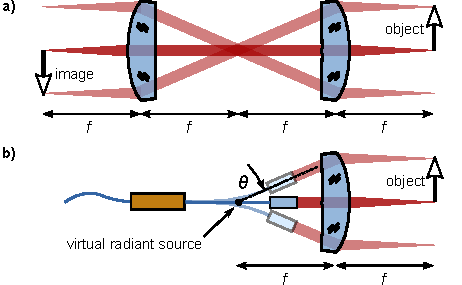
\includegraphics[width=\columnwidth]{figures/fps2.pdf}
      \caption{Working principle of the fourier plane fiber scanner.
      \textbf{a)} Illustration of a classical telecentric system. The height of the object is translated into an angle $\theta$ in the collimated region between the two lenses. This angle is again translated into a corresponding image height by the second lens.
      \textbf{b)} Illustration of the OCT beam path using a fiber scanner in first resonance mode. The movement of the GRIN lens due to the fiber scanner and the distance between the GRIN lens and the focusing lens creating the same optical behavior as it can be observed in a classical telecentric system.}
      \label{fig:fps}
\end{figure}



%%%%%%%%%%%%%%%%%%%%%%%%%%%%%%%%%%%%%%%%%%%%%%%%%%%%%%%%%%%%%%%%%%%%%%%%
\section{Mechanical design}
%%%%%%%%%%%%%%%%%%%%%%%%%%%%%%%%%%%%%%%%%%%%%%%%%%%%%%%%%%%%%%%%%%%%%%%%
Fiber scanners use mechanical resonance to amplify the subtle movement of a piezoelectric actuator into a large displacement of the tip of an optical fiber. As in any resonant system, the geometrical and mechanical characteristics of the flexible cantilever of the FPFS fully define its operating frequency range, and with it, constrain the way the object can be imaged. In the following paragraphs the behavior of the fiber scanner is mechanically modeled and this information used to choose the most relevant fabrication parameters leading to a resonant frequency adequate for OCT.

\subsection{Piezoelectric tube actuators}
\label{ssec:piezo}
A piezoelectric tube is a solid state actuator consisting of a tube made of radially polarized piezoelectric material with inner and outer electrodes. If a voltage difference is applied to two opposite electrodes of the tube, one side will contract while the other will expand due to the piezoelectric effect, inducing a deflection of the tip of the tube linear with the applied voltage. In case of bipolar operation, the deflection $\Delta y$ is estimated by \cite{Chen} as
\begin{equation}
\Delta y = V  \frac{2 \sqrt{2} d_{31} L^2}{\pi D h},
\end{equation}
where \textit{V} is the voltage applied to each opposing electrode, $d_{31}$ is the piezoelectric strain coefficient of the material in direction perpendicular to the polarization direction, \textit{L} is the length of the tube, \textit{D} its outer diameter and \textit{h} the thickness of its wall. Thus, longer tubes with a thinner diameter and wall thickness maximize the deflection of the tip. With these requirements, \textit{Physik Instrumente (PI) GmbH} was able to manufacture a piezoelectric tube with \SI{800}{\micro\meter} external diameter, \SI{500}{\micro\meter} internal diameter and \SI{3.7}{\milli\meter} long using PIC 151 piezoelectric material. The deflection of this actuator is in the order of $\SI{20}{\nano\meter / \volt}$.

\subsection{Analysis of the resonant beam}
\label{ssec:EB}
The piezoelectric actuator couples mechanical energy into the cantilever of the scanner formed by a optical fiber segment to which a GRIN lens is glued, as depicted in \autoref{fig:EB}a.

\begin{figure}[h!]\centering
      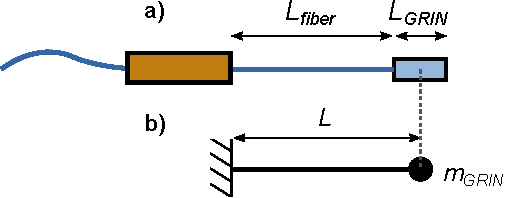
\includegraphics[width=6cm]{figures/EB.pdf}
      \caption{\textbf{a)} Schematic drawing of the piezoelectric scanner, composed of a piezoelectric tube, fiber and GRIN lens. 
      \textbf{b)} Simplified mechanical diagram obtained by modeling the fiber as a weightless cantilever and the GRIN lens as a point mass.}
      \label{fig:EB}
\end{figure}

The fiber-GRIN assembly can be modeled as a point-loaded, fixed-free cantilever where the weight of the GRIN lens is concentrated in its center of gravity, as represented in Figure \ref{fig:EB}b. 

Now, by applying the ideal mass-spring harmonic resonator equation, the resonance frequency can be estimated as 
\begin{equation}
f_\mathrm{res} = \frac{1}{2 \pi} \sqrt{\frac{K_\mathrm{cantilever}}{m_{\mathrm{GRIN}}}} 
\label{eq:fres}
\end{equation}
where $K_\mathrm{cantilever}$ represents the elastic constant of the fiber cantilever. Considering it as a fixed-free, point loaded cantilever, its spring constant can be calculated as 
\begin{equation}
K_\mathrm{cantilever} = \frac{3 E I}{L^3} = \frac{3 \pi}{4} \frac{E_\mathrm{fiber} r_\mathrm{fiber}^4}{L^3}
\label{eq:EB}
\end{equation}
following the Euler-Bernoulli theory \cite{MarcJ.Madou2011} and considering that the moment of inertia of the cylindrical fiber is given by $I_\mathrm{fiber} = \frac{\pi}{4} r^4$. 

This frequency 
\begin{equation}
f_\mathrm{res} = \frac{1}{2 \pi} \sqrt{\frac{3 \pi\ E_\mathrm{fiber}\ r_\mathrm{fiber}^4}{4\ L^3\ m_{\mathrm{GRIN}}}} 
\label{eq:fres}
\end{equation}
can be reduced in different ways: increasing the cantilever length $L$, decreasing the radius of the fiber $r_\mathrm{fiber}$ or increasing the mass at the tip $m_{\mathrm{GRIN}}$. First, by having a \SI{350}{\micro\meter} diameter, \SI{2.16}{\milli\meter} GRIN lens attached at the tip, the resonance frequency is reduced by a factor of 62\% when compared to a bare fiber scanner. Furthermore, by choosing a fiber with a cladding diameter of \SI{80}{\micro\meter} instead of the standard \SI{125}{\micro\meter}, the resonance frequency can be lowered by an extra factor of 60\%, as the sensitivity of the resonance frequency to the diameter of the fiber is quadratic. 

When selecting the length of the scanner, there are two details to consider. First, the maximum displacement of the \SI{350}{\micro\meter} GRIN lens is limited by the walls of the housing to usually a small deflection. Within that small displacement we want to achieve the maximum angular deflection of the GRIN lens to maximize the FOV. This can be achieved by using shorter fiber lengths, which induces a smaller radius of curvature. This exhibits a trade-off with the density of sampling $k_{sampling}$, which is increased with slower scanning coming from longer fiber. To balance those terms, a total scanner length of \SI{4.5}{\milli\meter} was chosen, which results in a resonance frequency of \SI{770}{\hertz} and a maximum angular deflection of \SI{5}{\degree}.


\subsection{COMSOL simulation}

In order to validate the theoretical analysis of the previous section, a multiphysics finite element analysis was performed using COMSOL. The actuator was modeled as a radially polarized piezoelectric material and the rest of the structure as fused silica. The excitation voltage is a sinusoidal symmetrical potential between the top and bottom electrodes of the tube. Note that, as the system undergoes small deflections, it is simulated assuming linear behavior without incurring in important deviations \cite{Fertis2006}.

As the first step, the resonant frequency of the system is simulated. An \textit{Eigenfrequency} study calculates the first mode resonance at \SI{762}{\hertz}, which closely matches the analytical estimation of \SI{770}{\hertz}. The mode shape at resonance is shown in Figure \ref{fig:defle}, where it can be observed that the actuator and the base of the fiber are almost static, confirming the resonant behavior of the scanner.

\begin{figure}[h!]\centering
      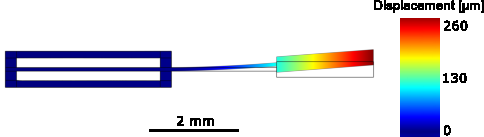
\includegraphics[width=\columnwidth]{figures/deflection.pdf}
      \caption{COMSOL simulation showing a cross section of the scanner maximum deflection at resonance for an actuation voltage of $\pm \SI{75}{\volt}$. The deformed structure is color coded showing the total displacement from the rest position (shown outlined). }
      \label{fig:defle}
\end{figure}

Note that, as the system is working close to resonance, it is challenging to simulate the oscillation amplitude, as it depends on its damping factor which should be obtained experimentally. Thus, for the simulation, this value was chosen to fit the expected deflection. 



%%%%%%%%%%%%%%%%%%%%%%%%%%%%%%%%%%%%%%%%%%%%%%%%%%%%%%%%%%%%%%%%%%%%%%%%
\section{Optical design}
%%%%%%%%%%%%%%%%%%%%%%%%%%%%%%%%%%%%%%%%%%%%%%%%%%%%%%%%%%%%%%%%%%%%%%%%

\subsection{Geometrical optics}
In a FPFS, the numerical apertures and focal lengths of the scanning and objective lens are related by the diameter of the beam in the intermediate region between both lenses. Thus, based on the schematic of Figure \ref{fig:opticsParam}, 
\begin{figure}[h]\centering
      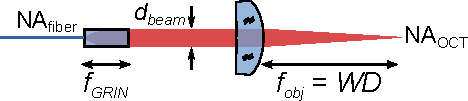
\includegraphics{figures/opticsParam.pdf}
      \caption{Optical diagram for the scanner at rest position indicating the main parameters.}
      \label{fig:opticsParam}
\end{figure}
the following geometrical optics relations are obtained: $d_\mathrm{beam} \simeq 2\cdot f_\mathrm{GRIN}\cdot \mathrm{NA}_\mathrm{fiber}$ and $d_\mathrm{beam} \simeq 2 \cdot f_\mathrm{obj}\cdot \mathrm{NA}_\mathrm{OCT}$. By combining them together, the main design equation for the scanner is obtained
\begin{equation}
f_\mathrm{GRIN} \cdot \mathrm{NA}_\mathrm{fiber} = f_\mathrm{obj} \cdot \mathrm{NA}_\mathrm{OCT}.
\label{eq:fpsNA}
\end{equation} Note that these equations use a small angle approximation valid for small NA:  $\tan[\sin^{-1}(\mathrm{NA})] \simeq \mathrm{NA} $. In this case, as any NA is smaller than 0.25, the error of this simplification is smaller than 2\%.

\subsection{Selection of components}
The only commercially available single mode fiber working in the necessary wavelength range and with thinned cladding diameter (refer to \autoref{ssec:EB}) is \textit{Thorlabs SM980G80}, with a diameter of \SI{80}{\micro\meter} and with $\mathrm{NA_\mathrm{fiber}} = 0.18$ at $\lambda = \SI{1.33}{\micro\meter}$. In order to collimate the output from the fiber without clipping the gaussian beam in excess, a GRIN lens with an $\mathrm{NA_{GRIN}}$ higher than $\mathrm{NA_{fiber}}$ is needed. GRINTECH \textit{GT-LFRL-035-024-20-CC (1550)} was chosen, with an $\mathrm{NA_\mathrm{GRIN}} = 0.20$ and $\mathit{f_\mathrm{GRIN}} = \SI{0.91}{\milli\meter}$. 

Now, by using the relation in \autoref{eq:fpsNA} we can design $f_\mathrm{objective}$ by choosing an adequate $\mathrm{NA_\mathrm{OCT}}$. By choosing an intermediate $\mathrm{NA_\mathrm{OCT}}$ of 0.022, the focal length of the objective lens can be selected by
\begin{equation}
\mathit{f_\mathrm{obj}} = f_\mathrm{GRIN}\ \frac{\mathrm{NA_\mathrm{fiber}}}{\mathrm{NA_\mathrm{OCT}}}  = \SI{0.91}{\milli\meter}\ \frac{0.18}{0.022} = \SI{7.5}{\milli\meter}.
\end{equation}

The field of view (FOV) can be now calculated considering the maximum angular deflection of the GRIN lens in the tip of the scanning fiber by 
\begin{equation}
h_\mathrm{max} = f_\mathrm{obj}\cdot \tan  \theta_\mathrm{max} = \SI{7.5}{\milli\meter} \cdot \tan \SI{5}{\degree} = \SI{0.66}{\milli\meter}, 
\end{equation}
equivalent to a FOV of \SI{1.2}{\milli\meter} for a $\theta_\mathrm{max} $ of $ \pm \SI{5}{\degree}$, as calculated in \autoref{ssec:EB}.

\subsection{Analysis of the lateral resolution}
\label{ssec:res}

Once the components and NA are chosen, it is of particular interest to calculate the expected lateral resolution of such a system.

To understand the optical modeling of a laser scanned imaging device such as OCT, the probe is first considered as an illumination device, i.e. a projector. In this case, laser light coming from the optical fiber will be focused by the optical system in an object plane located at its working distance. The focused spot won't be infinitesimally small due to two reasons: first, as in any optical system, diffraction takes place and blurs it with its $\textrm{PSF}_{\rm{optics}} (\mathbf{r})$, defined by the NA and the wavelength of the focused beam. Furthermore, the gaussian intensity distribution at the core of the fiber has a certain extent, characterized by its Mode Field Diameter (MFD). Once projected in the image plane, the MFD will be magnified by the optical system by a factor of $1/M$, where \textit{M} is the magnification of the beam defined as $f_\mathrm{fiber}/f_\mathrm{objective}$. This gaussian spot can be conceptually considered as the PSF due to the extended core of a fiber $\textrm{PSF}_{\rm{core}}$.

Thus, the projected spot can be considered as the illumination PSF, calculated by convolution as
\begin{equation}
\textrm{PSF}_{\rm{ill}}(\bm{r}) = \textrm{PSF}_{\rm{core}}(\bm{r}M) \ast \textrm{PSF}_{\rm{optics}} (\bm{r})
\end{equation}
or equivalently, the illumination MTF
\begin{equation}
\textrm{MTF}_{\rm{ill}}(\mathbf{k}) = \textrm{MTF}_{\rm{core}}(\bm{k}/M) \cdot \textrm{MTF}_{\rm{optics}} (\bm{k} )
\end{equation}
following the PSF-MTF relationship. This behavior can be observed in \autoref{fig:MTFcomplete}a, where $\textrm{MTF}_{\rm{core}}$ and $\textrm{MTF}_{\rm{optics}}$ are simulated according to the design values of this work.

\begin{figure}[h!]\centering 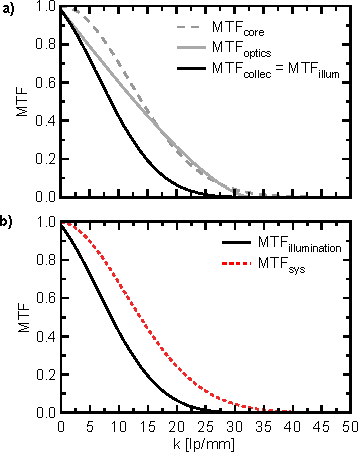
\includegraphics{figures/MTFcomplete.pdf}
      \caption{	\textbf{a)} Simulated MTF of the illumination or collection of a single point using the proposed optical system. The MTF is limited by the finite size of the fiber core and the diffraction of the optical system.
				\textbf{b)} MTF of the imaging system, calculated as the convolution of illumination and detection MTFs. The theoretical resolution of such a system according to the Rayleigh contrast $C_{Rayleigh}=0.152$ \cite{Blattmann}) is 23.3 line pairs/mm or \SI{43}{\micro\meter}.
				}
      \label{fig:MTFcomplete}
\end{figure}

The next step considers the detection or collection of the backscattered light. If all the light coming from the fiber is projected in the $\textrm{PSF}_{\rm{ill}}$, we can use the Helmholtz reciprocity property of light to state that the photons originating within this PSF will be collected by the fiber and detected by the photodiode. Thus, the detection PSF is equivalent to the illumination PSF,
\begin{eqnarray}
\textrm{PSF}_{\rm{det}}(\bm{r}) &= \textrm{PSF}_{\rm{ill}}(\bm{r}) =\\
&= \textrm{PSF}_{\rm{core}}(\bm{r}M) \ast \textrm{PSF}_{\rm{optics}} (\bm{r})
\end{eqnarray}
or equivalently,
\begin{eqnarray}
\textrm{MTF}_{\rm{det}}(\mathbf{k}) &= \textrm{MTF}_{\rm{ill}}(\mathbf{k})= \\
&=\textrm{ MTF}_{\rm{core}}(\bm{k}/M) \cdot \textrm{MTF}_{\rm{optics}} (\bm{k} )
\end{eqnarray}

Considering now the complete imaging process of a confocal laser scanning microscope, a photon traveling through the fiber is projected inside the $\textrm{PSF}_{\rm{ill}}$, with a higher probability of illuminating the focus position. After being scattered by the sample, it has a high probability of being collected by the detector, as it is also in the center of the $\textrm{PSF}_{\rm{det}}$. It can be concluded that both PSFs are multiplied together, and thus the complete imaging system \textit{PSF} given by 
\begin{equation}
\textrm{PSF}_{\rm{sys}}(\bm{r}) =\textrm{ PSF}_{\rm{ill}}(\bm{r}) \cdot \textrm{PSF}_{\rm{det}}(\bm{r}) \simeq \textrm{PSF}_{\rm{det}}(\bm{r})^2
\end{equation}
or equivalently, using the autocorrelation - squaring equivalence between spatial and frequency domain
\begin{eqnarray}
\textrm{MTF}_{\rm{sys}}(\mathbf{k}) &= \textrm{MTF}_{\rm{ill}}(\mathbf{k}) \ast \textrm{MTF}_{\rm{det}}(\mathbf{k}) &\simeq\\
&\simeq \textrm{AC}[\textrm{MTF}_{\rm{det}}(\mathbf{k})].
\end{eqnarray}
These operations are numerically calculated in \autoref{fig:MTFcomplete}b, leading to a theoretical resolution of 23.3 line pairs/mm or \SI{43}{\micro\meter}.



%%%%%%%%%%%%%%%%%%%%%%%%%%%%%%%%%%%%%%%%%%%%%%%%%%%%%%%%%%%%%%%%%%%%%%%%
\section{Spiral Scanning}
%%%%%%%%%%%%%%%%%%%%%%%%%%%%%%%%%%%%%%%%%%%%%%%%%%%%%%%%%%%%%%%%%%%%%%%%

The OCT optical setup samples the object at only a single point. Thus, the focus point has to be 2D-scanned over the surface of the sample to obtain 3D OCT images. When using fiber scanners, the movement of the scanning fiber is constrained to harmonic oscillations within a frequency close to its resonance frequency $f_\mathrm{res}$. This requirement limits the possible scanning patters to harmonic movements close to $f_\mathrm{res}$, excluding then raster scanning, which require at least an axis working out of resonance. Then, conventional alternatives are Lissajous \cite{Moon2010} and spiral scanning. In order to ease the reconstruction of the image, spiral scanning is implemented, which is described in the following paragraphs:

The piezoelectric tube which drives the scanner has four outer gold electrodes to control the lateral movement of the scanner, as described in \autoref{ssec:piezo}. Two independent voltage sources control the vertical and horizontal movement of the actuator by addressing the corresponding pair of electrodes. If sine and cosine signals of the same frequency $f_\mathrm{drive}$ are used to drive the scanner, the GRIN lens will oscillate in a circle of constant radius. If now the amplitude of these signals is amplitude modulated with another sinusoidal signal of frequency $f_\mathrm{mod}$, the resultant trajectory will be spiral, as illustrated in \autoref{fig:PZTDriving}.

\begin{figure}[h!]\centering 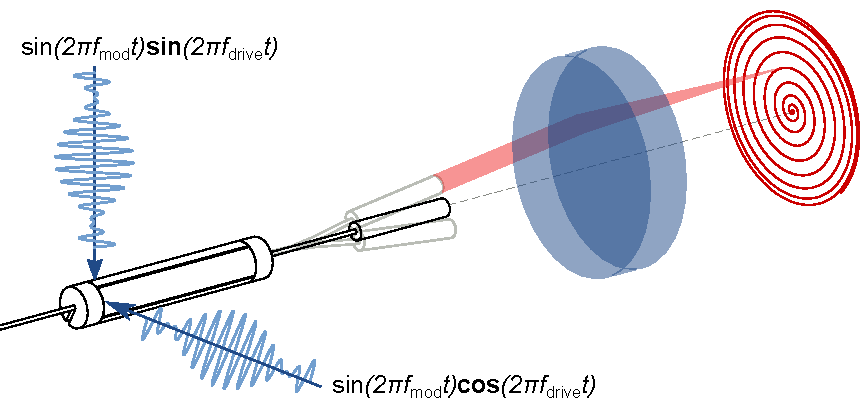
\includegraphics[width=\columnwidth]{figures/PZTDrivingMoving.pdf}
      \caption{Schematic of the piezoelectric tube, fiber, GRIN and objective lens focusing the OCT beam (red) in a plane. 
      The piezoelectric tube is driven with two independent amplitude modulated sine and cosine signals to generate a spiral pattern, used to acquire an image. The spiral trajectory has two different rings highlighted, where $n$ black dots represent the sampling points of each ring. Notice that in the inner ring the sampling density is higher than in the outer one.
      }
      \label{fig:PZTDriving}
\end{figure}


During the full period of the spiral pattern $T_\mathrm{spiral}=f_\mathrm{mod}^{-1}$ , two complete frames are acquired, one while the spiral grows, another while it shrinks. The whole pattern can be divided in $N_\mathrm{rings} = f_\mathrm{drive}/f_\mathrm{mod}$ individual rings, as depicted in \autoref{fig:PZTDriving}. The velocity at which the focus spot scans the image
\begin{equation}
v_\mathrm{spot} = 2 \pi r_\mathrm{ring} f_\mathrm{drive}
\end{equation}
depends on the driving frequency $f_\mathrm{drive}$ and the radius of the ring $r_\mathrm{ring}$. In order to fulfill the Nyquist theorem, this speed should be low enough so that the spatial sampling 
\begin{equation}
k_\mathrm{sampling} = \frac{f_\mathrm{sampling}}{v_\mathrm{spot}} = \frac{f_\mathrm{sampling}}{ 2\pi r \ f_\mathrm{drive}  }> 2\ k_\mathrm{opt}
\end{equation}
is at least double the optical bandwidth $k_\mathrm{opt}$. For a driving frequency $f_\mathrm{drive}$ of \SI{770}{\hertz} and a sampling rate 
$f_\mathrm{sampling} $ of \SI{100}{\kilo\hertz}, the image will be oversampled up to a field of view of \SI{0.89}{\milli\meter} and slightly undersampled outside this area.


%%%%%%%%%%%%%%%%%%%%%%%%%%%%%%%%%%%%%%%%%%%%%%%%%%%%%%%%%%%%%%%%%%%%%%%%
\section{Fabrication and assembly}
%%%%%%%%%%%%%%%%%%%%%%%%%%%%%%%%%%%%%%%%%%%%%%%%%%%%%%%%%%%%%%%%%%%%%%%%

This section details the implementation of the probe shown in \autoref{fig:exploded}, which serves as a demonstrator of the fiber scanner design and evaluation tool of the optical performance of the OCT beam path.

\begin{figure}[h!]\centering 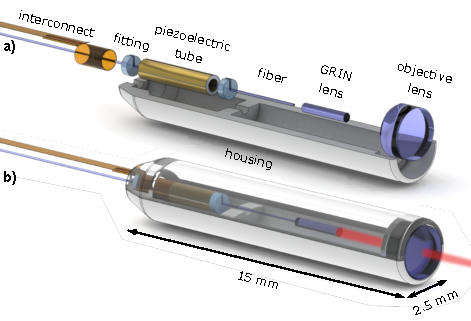
\includegraphics[width=\columnwidth]{figures/explodedRenderNames.pdf}
      \caption{\textbf{a)} Exploded view of the components which form the OCT endoscopic probe.
      \textbf{b)} Render of the complete probe after assembly, showing the laser path pointing to the sample.}
      \label{fig:exploded}
\end{figure}

The design can be summarized as follows: A polyimide ribbon cable is wrapped around the piezoelectric actuator to address its electrodes and control the lateral movement of the scanner. A single mode fiber is centered in the piezoelectric tube and the GRIN lens bonded to the tip of this fiber. This arrangement enables a compact fiber scanner with a total length of \SI{9}{\milli\meter} and a resonance frequency of \SI{750}{\hertz} optimized for an OCT system with an A-Scan repetition rate of \SI{100}{\kilo\hertz}. The scanner and the objective lens are then assembled in a 3D printed polymer housing.

\subsection{Polyimide electrodes}

Due to the small diameter of the tube (\SI{800}{\micro\meter}), creating a reliable interface between the driving circuit and its electrodes is not trivial. Other piezoscanner implementations use soft soldering and insulated copper wires \cite{Lee2010, Meinert, Huo2010}, but the soldering process can damage the piezoelectric material, as it is exposed to temperatures above its Curie temperature and also increases the diameter of the actuator significantly, as a solder blob is needed. %Furthermore, it requires welding by hand in a \SI{600}{\micro\meter} curved electrode.

Instead, this design uses a polyimide ribbon cable which is wrapped around the piezotube and addresses its four external electrodes using vias. Its geometry, cross section and application over the tube is depicted in Figure \ref{fig:piRolled}.

\begin{figure}[h!]\centering 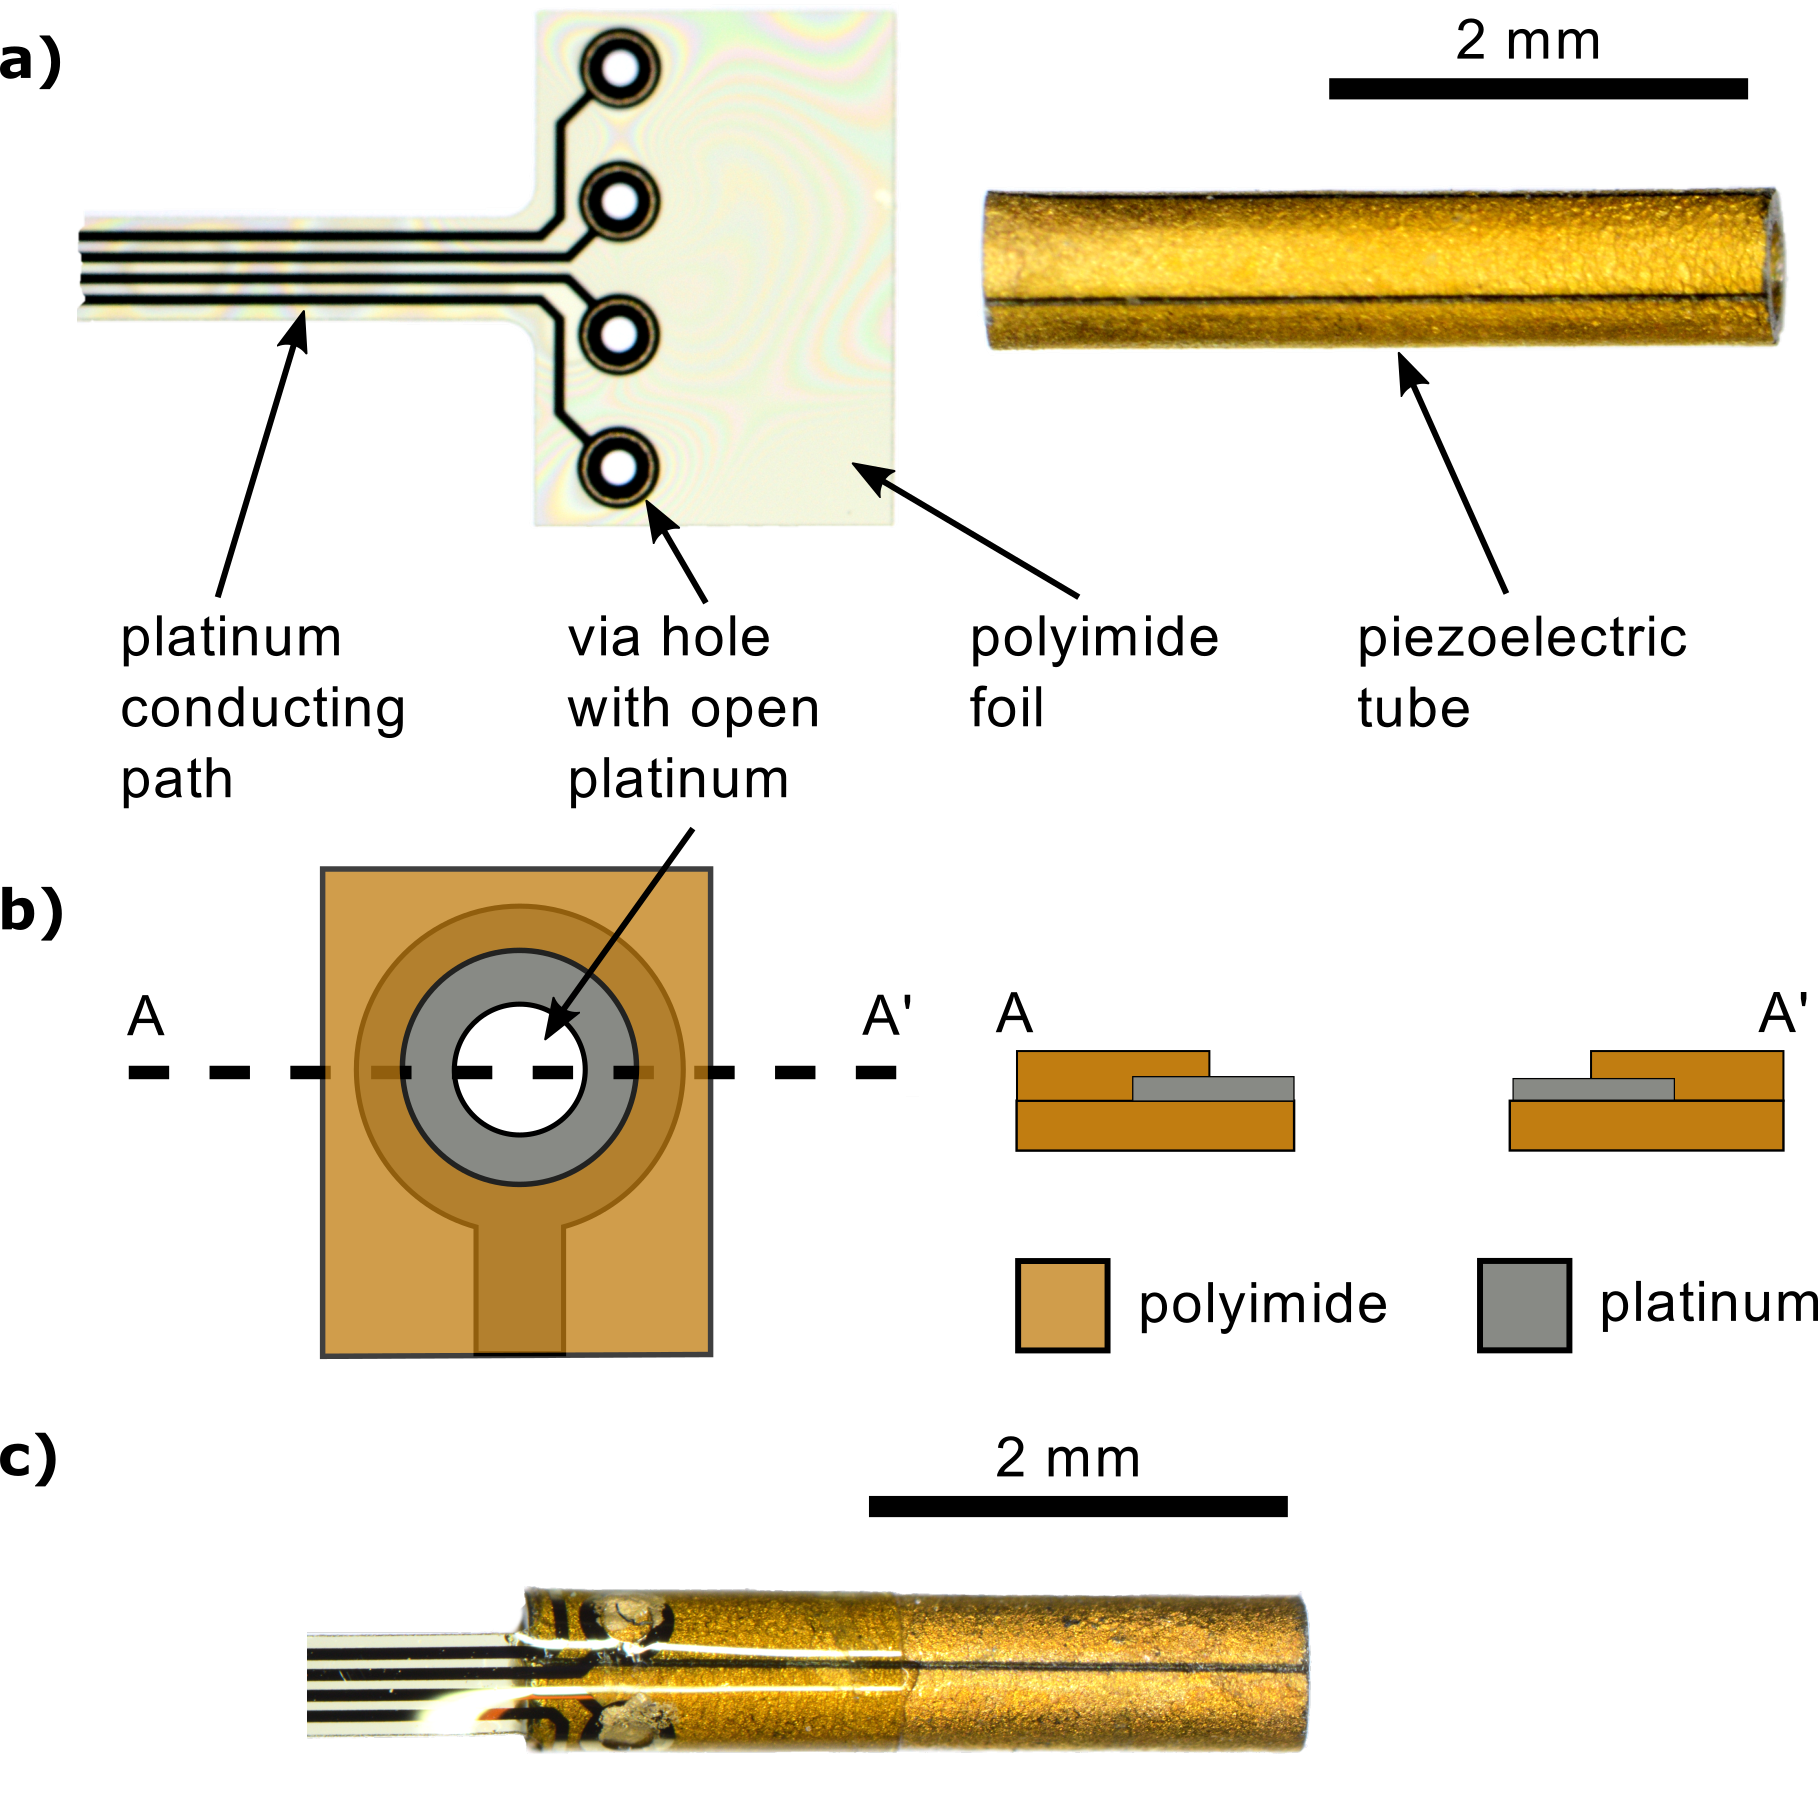
\includegraphics[width=\columnwidth]{figures/tubeFoil.png}
      \caption{Polyimide electrode design.
      \textbf{a)} \textit{Left}: Photo of the polyimide ribbon cable with four vias to contact the four gold electrodes of the piezoelectric tube. \textit{Right}: Piezoelectric tube.
      \textbf{b)} Schematic of one via and its cross section. The platinum around the via is partly uncovered to improve the electrical connection between the cable and the piezoelctric tube.
      \textbf{c)} Photography of a polyimide ribbon cable, wrapped around the piezoelectric tube that is electrical connected through the vias by conductive glue.}
      \label{fig:piRolled}
\end{figure}

The polyimide ribbon cables are manufactured using a cleanroom process summarized in \autoref{fig:PIprocess}. This process is similar to the one developed for cuff electrodes for nerve stimulation \cite{Rodriguez2000} and consists of platinum tracks and via holes embedded in a polyimide substrate. One end of the cable is shaped to fit a zero insertion force (ZIF) connector while the other end can be rolled around the piezoelectric tube, allowing the bonding to its gold electrodes using conductive glue (Araldite 2020 with 80\% wt. silver particles).

\begin{figure}[h!]\centering 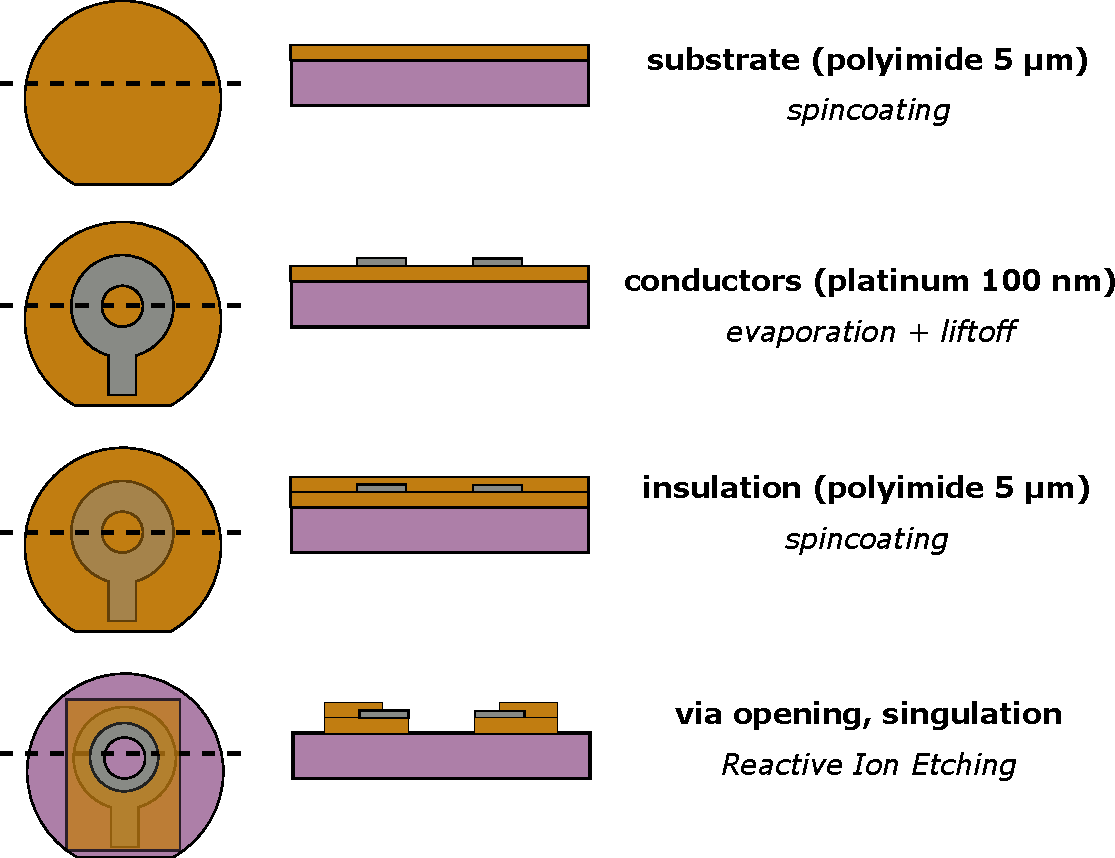
\includegraphics[width=\columnwidth]{figures/PIprocess.pdf}
      \caption{Simplified processing steps for the fabrication of a polyimide-platinum via. The first column shows the top view of the wafer, while the cross section is depicted in the second column.}
      \label{fig:PIprocess}
\end{figure}


\subsection{Fiber-GRIN bonding}
The bonding of a single mode, \SI{80}{\micro\meter} optical fiber to a GRIN lens was performed using a custom silicon microfabricated tool. This method allows a placement accuracy in the \SI{}{\micro\meter} range, creating an optical and mechanical bond that operates reliably under the high mechanical stress found in a resonant scanner. 

Prior OCT setups including GRIN lenses showed that they can cause problematic backreflections due to collimated incidence in the glass-air facet of the fiber. This problem was successfully avoided by a custom GRIN lens design with a \SI{1}{\degree} tilted exit facet. This solution, together with an special attention to the layout of the optical components, resulted in an optical system with backreflections below 0.02\%.


\subsection{Assembly}

The scanner and optical components are assembled in a 3D printed polymer structure that also acts as housing. A \textit{B9Creator} stereolithography printer together with a custom acrylic resin achieves a lateral resolution of \SI{30}{\micro\meter}.

The assembly is performed manually using the multiple alignment features of the housing. The exploded view in \autoref{fig:exploded} shows the placement of the components prior to assembly, followed by the final encapsulation. This process is summarized as follows:

\begin{enumerate}
\item The GRIN lens is aligned to the end of the fiber inside a micromachined silicon alignment tool and glued using index-matched optical adhesive.
\item The GRIN-fiber assembly is slid through the piezotube and centered with laser cut FR-2 fittings, which are glued to the piezotube using cyanocrilate.
\item The piezotube-fiber-GRIN assembly is placed in the bottom half of the housing and glued in place using cyanocrilate with help of the alignment structures.
\item The planoconvex lens is placed in the bottom half of the housing and glued using UV-curable optical glue.
\item The probe is closed with the top half of the housing and sealed with UV-curable glue.
\end{enumerate}


%%%%%%%%%%%%%%%%%%%%%%%%%%%%%%%%%%%%%%%%%%%%%%%%%%%%%%%%%%%%%%%%%%%%%%%%
\section{Experimental evaluation}
%%%%%%%%%%%%%%%%%%%%%%%%%%%%%%%%%%%%%%%%%%%%%%%%%%%%%%%%%%%%%%%%%%%%%%%%

\subsection{Dynamic behavior of the scanner}
\label{sec:whirling}

The dynamic behavior of the scanner was measured by driving the scanner with a sweeping sinusoidal signal to a pair of electrodes and observing the amplitude of its oscillation using a position sensitive detector (PSD). The result, plotted in \autoref{fig:bode}a, shows the expected resonant behavior, but reveals two different resonant frequencies, indicating that the resonant cantilever has two planes of symmetry or eigendirections with different stiffness. Close to resonance, they create a cross-plane instability in which excitation of the base of the resonator in the one eigendirection can lead to oscillations in the other eigendirection. This effect can be seen in the whirl plots of \autoref{fig:bode}b and was already identified in the first fiber scanner implementations \cite{Seibel2001}.


\begin{figure}[h!]\centering 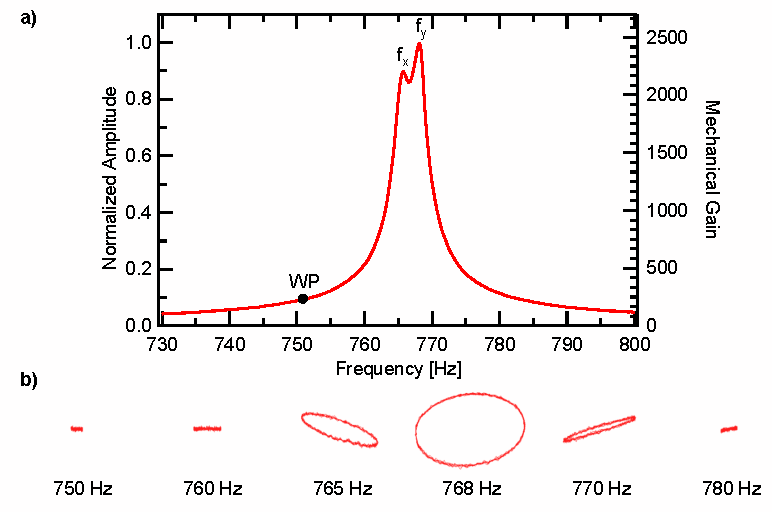
\includegraphics[width=\columnwidth]{figures/bodeWhirl.pdf}
      \caption{\textbf{a)} Dynamic behavior of the scanner under harmonic excitation. The two eigenfrequencies corresponding to the main axes of the scanner are marked as $f_\mathrm{x} = \SI{765.8}{\hertz}$ and $f_\mathrm{y} = \SI{768.1}{\hertz}$.
      The Working Point WP shows a gain of 220 at \SI{752}{\hertz}. 
      The right axis shows the mechanical gain due to resonance, defined as the ratio of the displacement of the GRIN tip to the displacement of the piezoelectric tube tip.
      \textbf{b)} Whirl patterns obtained by exciting the scanner in the $x$ direction with different harmonic frequencies while measuring the position of the fiber tip. }
      \label{fig:bode}
\end{figure}

In order to reduce the imaging distortions caused by whirling, the scanner operates at a working point \textit{WP} slightly away from the resonance, but with a high enough mechanical gain to achieve the required amplitude of oscillation.


\subsection{Laser scanning imaging}


It is possible to use the OCT probe and optical system to perform laser scanning imaging (LSI). This 2D imaging modality, analogous to confocal microscopy, is used to assess the lateral resolution and depth of field of the probe. As OCT uses the concept of LSI to recreate volumetric images, these results are also representative for OCT imaging.

LSI is accomplished by coupling light originating from a laser source to the probe through a circulator, which transfers the backscattered light from the sample to a photodetector. While the probe scans an object with a spiral pattern defined by the driving voltage datapoints $(\mathbf{u_x}[n], \mathbf{u_y}[n])$, the data acquisition system (DAQ) samples a stream of intensities at the photodetector $\mathbf{I}[n]$, as shown in \autoref{fig:confPlotting}a. As these signals are generated and acquired synchronously, we expect that the intensity $\mathbf{I}[i]$ corresponds to a point in object space linearly related to the driving voltage of the piezoelectric scanner: $(x, y) = K_\mathrm{mech}(\mathbf{u_x}[i], \mathbf{u_y}[i])$, where $K_\mathrm{mech}$ is a mechanical constant.

\begin{figure}[h!]\centering 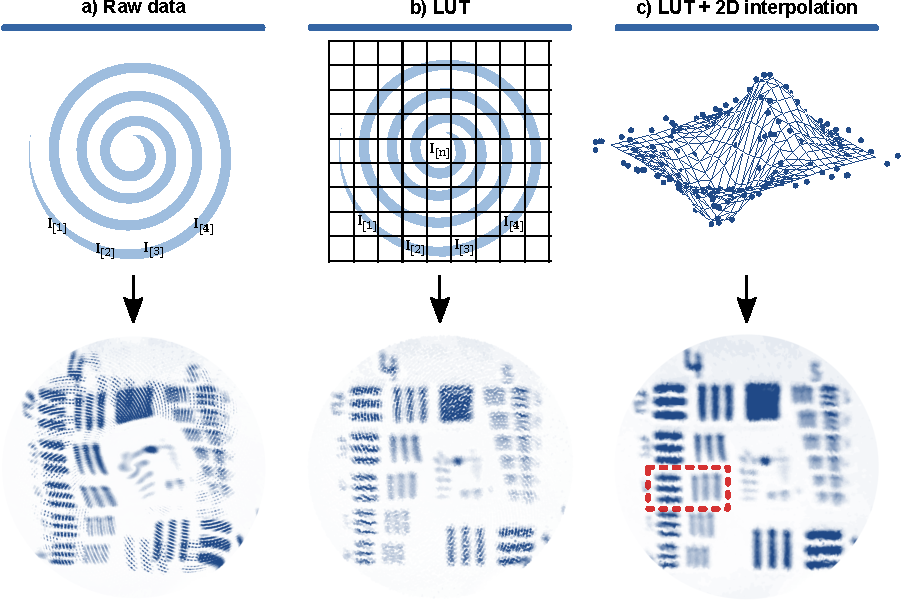
\includegraphics[width=\columnwidth]{figures/PlottingMark.pdf}
      \caption{Different representations of the same acquired datapoints $\mathbf{I}[n]$ of a USAF 1951 resolution test chart. The full acquired spiral consists of 374 rings of 122 datapoints, adding up to 45500 datapoints measured at \SI{91}{\kilo\hertz} during \SI{500}{\milli\second}. The field of view is \SI{1.1}{\milli\meter}.
      \textbf{a}: Point cloud assuming ideal movement of the scanner.
      \textbf{b}: Point cloud after correcting the position of each dot using a lookup table.
      \textbf{c}: Raster image after performing a 2D interpolation from the data in d. Element 4 of group 4 of the USAF target is marked with a dashed line.}
      \label{fig:confPlotting}
\end{figure}


\autoref{fig:confPlotting}a shows the image formed if all the datapoints $\mathbf{I}_{[n]}$ acquired during a full spiral are plotted as an intensity-coded dot located at the position $K_\mathrm{mech}(\mathbf{u_x}[n], \mathbf{u_y}[n])$. The distortion which can be seen in this image proves that the previous assumption of linearity is not valid, and thus the relationship between $(\mathbf{u_x}[i], \mathbf{u_y}[i])$ and $(\mathbf{x}[i], \mathbf{y}[i])$ is neither linear nor simple. This is the result of whirling, as discussed in \autoref{sec:whirling}. There are two general methods to overcome this problem:

The first one involves closed loop operation, where the current position of the scanner is measured inside the probe and used by the plotting system to correct for the distortion \cite{Yeoh2014}. 

The open loop alternative, used in this demonstrator, assumes that the distortion pattern is constant for a given driving signal. Then, the distorted spiral pattern $(x[i], y[i])$ can be measured after the assembly of the probe using a position sensitive device (PSD) and stored as a calibration lookup table.
Once this calibration step is performed, any further frame is plotted by assigning a position $(\mathbf{x}[i], \mathbf{y}[i])$ to every measured intensity $\mathbf{I}[n]$, as depicted in \autoref{fig:confPlotting}b, resulting in a dot plot with less distortion. This procedure can be performed in real time.

The dot plots which are obtained from spiral scanners have the inconvenient of non-uniform sampling, as can be seen in \autoref{fig:confPlotting}b. Thus, to ease the further processing of the acquired images, it is beneficial to convert the non-uniform dot plot into a cartesian raster image. This can be performed by 2D interpolation, resulting in \autoref{fig:confPlotting}c.


\subsection{Lateral resolution measurement}
The optical performance of the scanner is qualitatively evaluated by capturing a SLI image of a USAF 1951 resolution test chart with a spiral scanning pattern. As can be seen in \autoref{fig:confPlotting}c, element 4 of group 4 is resolved, indicating a resolution of 22 line pairs/mm or \SI{45}{\micro\meter}. 
%
%\begin{figure}[h!]\centering 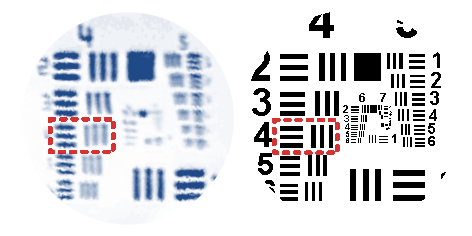
\includegraphics[width=\columnwidth]{figures/USAF.pdf}
%      \caption{Simplified processing steps for the fabrication of a polyimide-platinum via. The first column shows the top view of the wafer, while the cross section is depicted in the second column.}
%      \label{fig:USAF}
%\end{figure}

A more robust measurement of the optical resolution, independent from the scanning speed and patter can be obtained by manually scanning the focus of the probe over a sharp chromium edge of the test chart. This way the edge spread function (ESF) is obtained. By performing a spatial derivative followed by a Fourier transform of the ESF, the MTF can be obtained, plotted in \autoref{fig:MTF}b. Based on this curve the lateral resolution of the OCT beam path was determined at 21 line pairs/mm or \SI{47.6}{\micro\meter}. This value shows a good agreement with the theoretical resolution, calculated in \autoref{ssec:res} as 23.3 line pairs/mm or \SI{43}{\micro\meter}. The 10\% deviation between these values can be explained by small misalignments of the optical components induced by the process tolerances of the 3D-printed housing and the assembly process.
\begin{figure}[h!]\centering 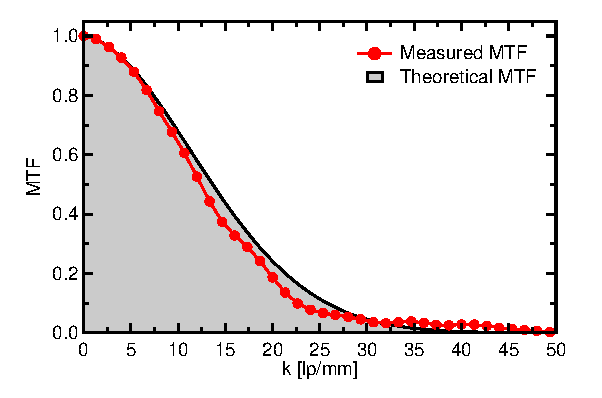
\includegraphics[width=\columnwidth]{figures/confRes.pdf}
      \caption{Experimental MTF obtained from the ESF compared with the theorical limit using the theory from \autoref{ssec:res}.}
      \label{fig:MTF}
\end{figure}


\subsection{Depth of field measurement}
The depth of field (DOF) of the OCT imaging system can me determined by measuring how much light is backreflected upon a mirror while displacing it though the z axis. The results from this experiment are plotted in \autoref{fig:FWHM}, where a full width half maximum (FWHM) DOF of \SI{3.5}{\milli\meter} is calculated. 

\begin{figure}[h!]\centering 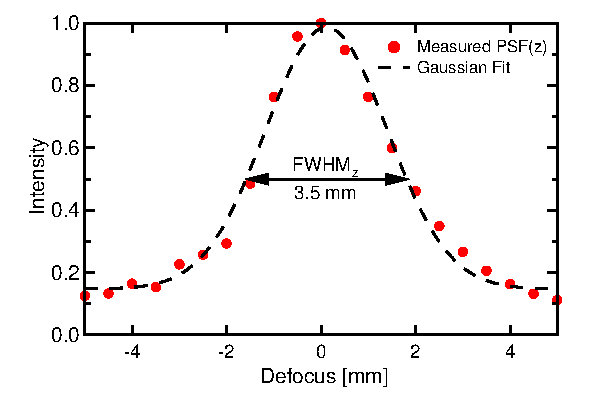
\includegraphics[width=\columnwidth]{figures/PSFz.pdf}
      \caption{Measurement of the axial resolution of the single modality probe. The intensity of the light coupled back into the optical system after reflection on a mirror is plotted against the manual translation of the mirror by $\pm \SI{4.5}{\milli\meter}$ from the focal plane of the probe. }
      \label{fig:FWHM}
\end{figure}




\subsection{OCT imaging}

First OCT test were performed using a swept-source OCT system property of the Medical University Vienna. This systemoperates with a center wavelength of \unit[1.34]{$\mu$m}, a bandwidth of \unit[37]{nm} and a theoretical axial resolution in air of \unit[26.9]{$\mu$m}.

Circular B-Scans of a colon polyp and a fingertip were captured with the single modality demonstrator, shown in \autoref{fig:B-Scan}. 
\begin{figure}[h!]\centering \includegraphics[width=\columnwidth]{figures/OCT_Measurement_arrangement}
      \caption{a) Illustration of the measurement arrangement for the circular B-Scan used as a proof of concept of OCT. b) Image of a circular OCT B-Scan of a colon polyp with a diameter $d=0.8\,\text{mm}$. Structural changes within the tissue can be detected and at the current state of the investigation the images suggest that blood vessels can be detected.
      c) Image of a circular OCT B-Scan of a human finger tip, where the epidermis, dermis and hypodermis can be tentatively differentiated.}
      \label{fig:B-Scan}
\end{figure}

These preliminary results prove that OCT imaging is possible. But at the same time, the low SNR of these images indicate that the designed system, which has a NA of 0.022, has problems collecting enough backscattered light while scanning. Therefore, future implementations of the probe could benefit from a higher NA. In that case, the resolution and collection of light of the system would be increased at the cost of a shorter working distance and a shorter depth of field. 



%%%%%%%%%%%%%%%%%%%%%%%%%%%%%%%%%%%%%%%%%%%%%%%%%%%%%%%%%%%%%%%%%%%%%%%%
\section{Discussion}
%%%%%%%%%%%%%%%%%%%%%%%%%%%%%%%%%%%%%%%%%%%%%%%%%%%%%%%%%%%%%%%%%%%%%%%%


%%%%%%%%%%%%%%%%%%%%%%%%%%%%%%%%%%%%%%%%%%%%%%%%%%%%%%%%%%%%%%%%%%%%%%%%
\section{Conclusion}
%%%%%%%%%%%%%%%%%%%%%%%%%%%%%%%%%%%%%%%%%%%%%%%%%%%%%%%%%%%%%%%%%%%%%%%%

The main goal of this work was the realization of a novel fiber scanner optimized for 3D OCT imaging. The complete scanning engine has an outer diameter of \SI{0.9}{\milli\meter} and a length of \SI{9}{\milli\meter}, and features custom fabricated \SI{10}{\micro\meter} thick polyimide flexible interconnect lines to address the four piezoelectric electrodes. This scanning engine was tested in a single modality, demonstrator probe with an external diameter of \SI{2.5}{\milli\meter} and a total length of \SI{15}{\milli\meter}, allowing the OCT imaging of a \SI{1}{\milli\meter} field of view with a resolution of \SI{45}{\micro\meter} using \SI{1330}{\nano\meter} light. 

To the best of our knowledge, the presented demonstrator probe is one of the most compact implementation of an OCT microendoscope.

During this project, the behavior of fiber scanners was analyzed and several approaches were discussed and simulated. It was concluded that its implementation as fourier plane scanner using a GRIN lens as collimator and weight was optimal for OCT. A complete electro-mechano-optical analysis and simulation followed, allowing the optimization of the system to reach diffraction-limited resolution and a maximized field of view.

Due to the small diameter of the piezoelectric tube used for the actuation (\SI{800}{\micro\meter}), the interface between the driving circuit and its electrodes involved the fabrication of a novel \SI{10}{\micro\meter} thick polyimide ribbon cable that can be rolled around the tube and contacted to it using vias and conductive glue.

The assembly of the demonstrator probe was successfully achieved using alignment features integrated in a 3D-printed housing. This part was manufactured using a commercial, low cost stereolithographic resin printer that enabled quick iterations of the design. 

Experimental measurements performed with the manufactured probe helped refining the assumptions used in the analytical calculation of the resolution of OCT systems. The resultant theoretical description, which closely matches experimental results, will help in the design of future OCT and confocal systems. Furthermore, the calibration method used in this work, which can operate in real time, reduces the imaging distortions to a minimum and enables the quantitative analysis of the acquired image. This enabled going one step further in cooperation with the Medical University Vienna, where the OCT imaging concept was proven. 

%%%%%%%%%%%%%%%%%%%%%%%%%%%%%%%%%%%%%%%%%%%%%%%%%%%%%%%%%%%%%%%%%%%%%%%%
\section*{References}
%%%%%%%%%%%%%%%%%%%%%%%%%%%%%%%%%%%%%%%%%%%%%%%%%%%%%%%%%%%%%%%%%%%%%%%%


\bibliographystyle{ieeetr}
\bibliography{refs}


%///////////////////////////////////////////////////////////////////////
%///////////////////////////////////////////////////////////////////////
\end{document}
%///////////////////////////////////////////////////////////////////////
%///////////////////////////////////////////////////////////////////////


Endoscopic methods play an increasingly important role in modern medicine. In general, the goal of endoscopy is to obtain as much information as possible for a viable diagnosis. To further improve diagnostics, there is a clear tendency towards multi-modal imaging by combining different imaging techniques. Making use of microscopy and Optical Coherence Tomography (OCT) in a single device is a promising approach to gather additional information and to thereby improve clinical diagnostics. 

The main goal of this work is the realization of a novel fiber scanner for 3D OCT imaging, designed for its combination with a full field microscope to form a multimodal probe. A tubular piezoelectric fiber scanner is used to perform en face scanning required for 3D OCT measurements. The complete scanning engine has an outer diameter of \SI{0.9}{\milli\meter} and a length of \SI{9}{\milli\meter}, and features custom fabricated \SI{10}{\micro\meter} thick polyimide flexible interconnect lines to address the four piezoelectric electrodes. To the best of our knowledge, the presented probe is one of the most compact implementation of an OCT microendoscope.

Optical and mechanical characterization of the scanner, implemented in a single modality demonstrator probe, show a high correlation with the analytical calculations and simulations. Thus, the approach described in this work constitutes a blueprint for a wide range of future scanning imaging probes.


This thesis realizes a novel fiber scanner in a telecentric configuration which reduce the distortion in the OCT modality and enables its integration within a multi-modal probe with dimensions of $13 \times 2 \times \SI{3}{\milli\meter^3}$. The complete scanning engine has an outer diameter of \SI{0.9}{\milli\meter} and a length of \SI{9}{\milli\meter}, and features custom fabricated \SI{10}{\micro\meter} thick polyimide flexible interconnect lines to address the four piezoelectric electrodes. The small cross section of the probe combined with its short length enables its use in a wide gamut of lumens in form of flexible or tilting head endoscope.

A single modality probe was designed to independently investigate the performance of the OCT beampath. This probe, depicted in \ref{fig:approachSketch}a, has an external diameter of \SI{2.5}{\milli\meter} and a total length of \SI{15}{\milli\meter}. Its optical design emulates that of the multimodal probe OCT path, enabling a direct translation of the results from this demonstrator probe to the multimodal one. To the best of our knowledge, this single modality probe is also one of the most compact implementation of an OCT microendoscope.

Using the demonstrator probe, it was possible to obtain preliminary \textit{en face} (\ref{fig:approachSketch}b) and tomographic (\ref{fig:approachSketch}c) images within a cylindrical volume of \SI{1}{\milli\meter} diameter and \SI{3}{\milli\meter} depth.


\section{Conclusion \& Outlook}

%The main goal of this work was the realization of a novel single-fiber-based scanning scheme enabling simultaneous 3D OCT in combination with full field microscopy using spectrally separated beampaths in a probe with dimensions of only $13 \times 2 \times \SI{3}{\milli\meter^3}$. 



\section{Conclusion}



